\documentclass[a4paper,10pt,twocolumn]{ltjarticle}
\usepackage{kaitoushu}

\pgfplotsset{
  myaxis/.style={
    axis lines=middle,
    xlabel={$x$}, ylabel={$y$},
    every axis x label/.style={at={(ticklabel* cs:1)},anchor=west},
    every axis y label/.style={at={(ticklabel* cs:1)},anchor=south},
    tick label style={font=\scriptsize},
    label style={font=\small},
    width=5.5cm, height=5cm,
    grid=none,
    samples=200,
  }
}

\begin{document}

\problemrange{5章：三角関数 — Check (p.65)（問300--308）}



\mondai{300}{次の角を弧度法で表せ．}
\kotae{
(1) $40°=\dfrac{2\pi}{9}$\quad (2) $50°=\dfrac{5\pi}{18}$\quad (3) $-18°=-\dfrac{\pi}{10}$\quad (4) $-210°=-\dfrac{7\pi}{6}$
}

\mondai{301}{次の角を60分法で表せ．}
\kotae{
(1) $\dfrac{7\pi}{6}=210°$\quad (2) $\dfrac{5\pi}{3}=300°$\quad (3) $-\dfrac{4\pi}{9}=-80°$\quad (4) $-\dfrac{11\pi}{4}=-495°$
}

\mondai{302}{半径6，中心角$\dfrac{5\pi}{6}$の扇形の弧の長さ$l$と面積$S$を求めよ．}
\kotae{
$l=6\cdot\dfrac{5\pi}{6}=5\pi$，$S=\dfrac{1}{2}\cdot36\cdot\dfrac{5\pi}{6}=15\pi$
}

\mondai{303}{次の三角関数の値を求めよ．}
\kotae{
(1) $\sin\dfrac{11\pi}{6}=\sin\!\left(2\pi-\dfrac{\pi}{6}\right)=-\sin\dfrac{\pi}{6}=-\dfrac{1}{2}$

(2) $\cos\!\left(-\dfrac{5\pi}{4}\right)=\cos\dfrac{5\pi}{4}=-\cos\dfrac{\pi}{4}=-\dfrac{\sqrt{2}}{2}$

(3) $\tan\!\left(-\dfrac{5\pi}{3}\right)=\tan\!\left(-\dfrac{5\pi}{3}+2\pi\right)=\tan\dfrac{\pi}{3}=\sqrt{3}$
}

\mondai{304}{$\theta$が第2象限で$\sin\theta=\dfrac{2}{3}$のとき，$\cos\theta$，$\tan\theta$を求めよ．}
\kotae{
$\cos^{2}\theta=1-\dfrac{4}{9}=\dfrac{5}{9}$．第2象限で$\cos<0$：$\cos\theta=-\dfrac{\sqrt{5}}{3}$

$\tan\theta=\dfrac{2/3}{-\sqrt{5}/3}=-\dfrac{2}{\sqrt{5}}=-\dfrac{2\sqrt{5}}{5}$
}

\mondai{305}{次の式を簡単にせよ．}
\kotae{
(1) $\sin(\pi+\theta)\cos(2\pi-\theta)+\sin\!\left(\dfrac{\pi}{2}+\theta\right)\cos(\pi-\theta)$

$=(-\sin\theta)(\cos\theta)+(\cos\theta)(-\cos\theta)=-\sin\theta\cos\theta-\cos^{2}\theta$

$=-\cos\theta(\sin\theta+\cos\theta)$

(2) $\dfrac{\sin(\pi-\theta)}{\cos\!\left(\frac{\pi}{2}+\theta\right)}-\dfrac{\tan(\pi+\theta)\cos(\pi+\theta)}{\sin\!\left(\frac{3\pi}{2}-\theta\right)}$

$=\dfrac{\sin\theta}{-\sin\theta}-\dfrac{\tan\theta\cdot(-\cos\theta)}{-\cos\theta}=-1-\tan\theta$
}

\mondai{306}{次の等式を証明せよ．}
\kotae{
(1) $\dfrac{1}{1+\sin\theta}+\dfrac{1}{1-\sin\theta}=\dfrac{2}{\cos^{2}\theta}$

左辺$=\dfrac{(1-\sin\theta)+(1+\sin\theta)}{1-\sin^{2}\theta}=\dfrac{2}{\cos^{2}\theta}=$右辺 \qed

(2) $\sin^{4}\theta-\cos^{4}\theta=\sin^{2}\theta-\cos^{2}\theta$

左辺$=(\sin^{2}\theta+\cos^{2}\theta)(\sin^{2}\theta-\cos^{2}\theta)=1\cdot(\sin^{2}\theta-\cos^{2}\theta)=$右辺 \qed
}

\mondai{307}{次の関数の周期とグラフをかけ．}
\kotae{
(1) $y=3\sin x$\quad 周期$2\pi$，振幅$3$

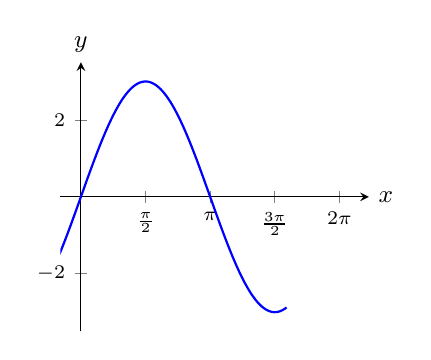
\begin{tikzpicture}
\begin{axis}[myaxis, xmin=-0.5,xmax=7,ymin=-3.5,ymax=3.5,
  xtick={1.5708,3.1416,4.7124,6.2832},
  xticklabels={$\frac{\pi}{2}$,$\pi$,$\frac{3\pi}{2}$,$2\pi$}]
\addplot[thick,blue]{3*sin(deg(x))};
\end{axis}
\end{tikzpicture}

(2) $y=\sin 3x$\quad 周期$\dfrac{2\pi}{3}$

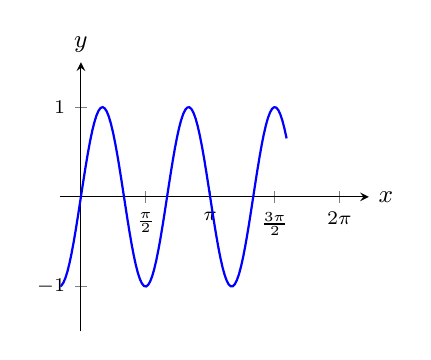
\begin{tikzpicture}
\begin{axis}[myaxis, xmin=-0.5,xmax=7,ymin=-1.5,ymax=1.5,
  xtick={1.5708,3.1416,4.7124,6.2832},
  xticklabels={$\frac{\pi}{2}$,$\pi$,$\frac{3\pi}{2}$,$2\pi$}]
\addplot[thick,blue]{sin(deg(3*x))};
\end{axis}
\end{tikzpicture}

(3) $y=\cos\!\left(x-\dfrac{\pi}{3}\right)$\quad 周期$2\pi$

\begin{tikzpicture}
\begin{axis}[myaxis, xmin=-0.5,xmax=7,ymin=-1.5,ymax=1.5,
  xtick={1.5708,3.1416,4.7124,6.2832},
  xticklabels={$\frac{\pi}{2}$,$\pi$,$\frac{3\pi}{2}$,$2\pi$}]
\addplot[thick,blue]{cos(deg(x-1.0472))};
\end{axis}
\end{tikzpicture}
}

\mondai{308}{$0\leqq x<2\pi$ で次を解け．}
\kotae{
(1) $2\cos x+\sqrt{3}=0$ → $\cos x=-\dfrac{\sqrt{3}}{2}$

$x=\dfrac{5\pi}{6},\;\dfrac{7\pi}{6}$

(2) $\tan x+1\geqq0$ → $\tan x\geqq-1$

$\tan x=-1$ となるのは $x=\dfrac{3\pi}{4},\;\dfrac{7\pi}{4}$

$\therefore 0\leqq x<\dfrac{\pi}{2}$ または $\dfrac{3\pi}{4}\leqq x<\dfrac{3\pi}{2}$ または $\dfrac{7\pi}{4}\leqq x<2\pi$

（$\tan$ の定義域に注意：$x\neq\dfrac{\pi}{2},\;\dfrac{3\pi}{2}$）
}

\end{document}
